% !TEX root = ../main.tex

\chapter{相关研究工作与关键技术基础}

本章沿 FlashTOD 的执行链路梳理相关工作，讨论的重点落在判断已有方法解决了哪一段问题、能够提供什么能力，以及这些能力接入候选召回---异常评分链路后还留下哪些系统边界。

\section{异常检测方法研究现状}

异常检测方法通常包括距离型、密度型、统计型、集成型和深度学习型路线\citep{chandola2009survey,markou2003novelty,aggarwal2017outlier}。对于金融数据来说，单笔交易偏离、账户时间窗行为变化和多实体关系异常的表现形式不同，处理方法的选择不能只看离线精度。评分计算复杂度、近邻依赖、GPU 批处理适配性、可解释性和在线维护代价都是影响系统能否进入近实时链路需要考虑的地方\citep{phua2010fraudsurvey,akoglu2015graph,song2024financialriskstgnn}。

$k$NN、LOF 和 ABOD 等方法依赖距离或邻域结构。$k$NN 需要计算并筛选近邻，LOF 还要在局部邻域上比较密度，ABOD 则通过样本对之间夹角的方差衡量离群程度\citep{breunig2000lof,angiulli2002fast,kriegel2008abod}。这类评分与偏离正常行为的业务解释较为接近，\texttt{cdist}、\texttt{topk} 和局部聚合也便于组织为 GPU 批处理；代价是近邻计算会随样本规模迅速增长\citep{zhao2022tod}。输入向量可能不大，全量距离矩阵和成对差分张量却可能先耗尽显存。候选召回因此不仅是检索加速手段，也是在进入这些评分方法前控制中间结果规模的系统约束。

HBOS、COPOD 和 ECOD 等统计型方法通常不需要维护完整近邻结构，单次评分较轻，适合快速基线或辅助筛查。COPOD 以经验 copula 估计多维尾部概率，ECOD 则直接从各维经验累积分布的尾部构造异常分数\citep{li2020copod,li2023ecod}。它们的代价同样明确：边缘分布、直方图或分位统计难以覆盖所有关系型和局部结构异常，对特征预处理与分布表达也更敏感。密度型方法处在两者之间，局部解释较直观，但近邻构造和邻域聚合仍然昂贵。表~\ref{tab:ad-complexity}用于集中展示这些取舍。

集成方法通过多个检测器或子空间模型提高稳健性，却会叠加推理成本与结果组织复杂度。Isolation Forest 通过随机切分形成多棵隔离树，较短的平均路径对应更容易被孤立的样本，是不依赖全量近邻矩阵的代表性集成方法\citep{liu2008isolationforest}。深度模型能够表达非线性、时序和图关系模式，但训练、部署和在线解释成本更高。以比特币反洗钱图数据研究和 CARE-GNN 为例，关系建模可以利用交易网络及异质邻居信息，同时也受到标签不平衡、噪声联系和数据构建方式影响\citep{weber2019bitcoinaml,dou2020caregnn,chen2021graphanomaly,li2023gnnfraud,yu2024rwkgnn}。这些方法适合不同任务，不能仅因模型复杂就认定更适合高吞吐部署。

本文不沿“最先进异常检测模型竞争”的路线展开。研究对象是系统协同：选择能够张量化的异常评分，把它放在规模受控的候选集合上运行，并观察效果与系统开销之间的折中。该边界保留了评分方法的可替换性，也避免将 FlashTOD 的系统收益解释为某个新检测模型的贡献。

\begin{table}[htbp]
  \caption{各类异常检测方法复杂度与系统适配性比较}
  \label{tab:ad-complexity}
  \centering
  \small
  \setlength{\tabcolsep}{3pt}
  \renewcommand{\arraystretch}{1.25}
  \begin{tabularx}{\linewidth}{@{}P{1.65cm}P{2.55cm}Y P{1.7cm}Y@{}}
    \toprule
    方法类别 & 代表方法 & 计算与部署取舍 & 可解释性 & 与候选召回的衔接 \\
    \midrule
    距离型 & $k$NN、ABOD、COF & 依赖距离和排序，GPU 批处理适配较好，但全量中间结果开销高 & 强 & 候选集合可直接限制距离计算范围 \\
    密度型 & LOF、LOCI & 需要近邻结构与局部聚合，邻域组织成本随规模增长 & 较强 & 可在候选邻域上评分，但依赖候选覆盖 \\
    统计型 & HBOS、COPOD、ECOD & 单次评分较轻，对预处理和分布表达较敏感 & 中等 & 可直接用于候选评分或快速基线 \\
    集成型 & Isolation Forest、特征装袋、检测器集成 & 不依赖完整近邻结构，多个评分器仍会增加推理和结果组织开销 & 中等 & 能够衔接，但候选集上仍需执行多个检测器 \\
    深度学习型 & Autoencoder、GNN、时序模型 & 表达能力强，训练、部署和在线维护成本较高 & 较弱 & 需要额外模型接口，超出本文评分主线 \\
    \bottomrule
  \end{tabularx}
\end{table}

\section{TOD/PyTOD 的 GPU 张量化执行基础}

TOD 解决的是异常评分如何统一映射到 GPU。它把算法拆为基础张量算子（Basic Tensor Operations，BTO）和由基础算子组成的功能算子（Functional Operations，FO），再用这些算子表达具体检测器\citep{zhao2022tod}。以 $k$NN 类评分为例，一条典型算子链可以写成 \texttt{cdist} $\rightarrow$ \texttt{topk} $\rightarrow$ local aggregation $\rightarrow$ anomaly score。距离、近邻筛选和聚合共享统一张量表示后，不再需要为每个检测器单独维护一套 GPU 实现。

图~\ref{fig:tod-overview}展示 TOD 的分层结构，图~\ref{fig:algo-to-ops}给出典型算法到算子的映射。自动批处理把超出显存预算的评分任务拆为可执行批次；可证明量化在其约束内压缩部分算子开销；多 GPU 支持允许批处理任务分配到多个设备。这些机制提高的是评分阶段的可执行性。它们并不改变 $k$NN、LOF 等方法对距离和邻域的基本依赖，也不能取消候选预算与检测效果之间的取舍\citep{zhao2022tod}。

\begin{figure}[!htbp]
  \centering
  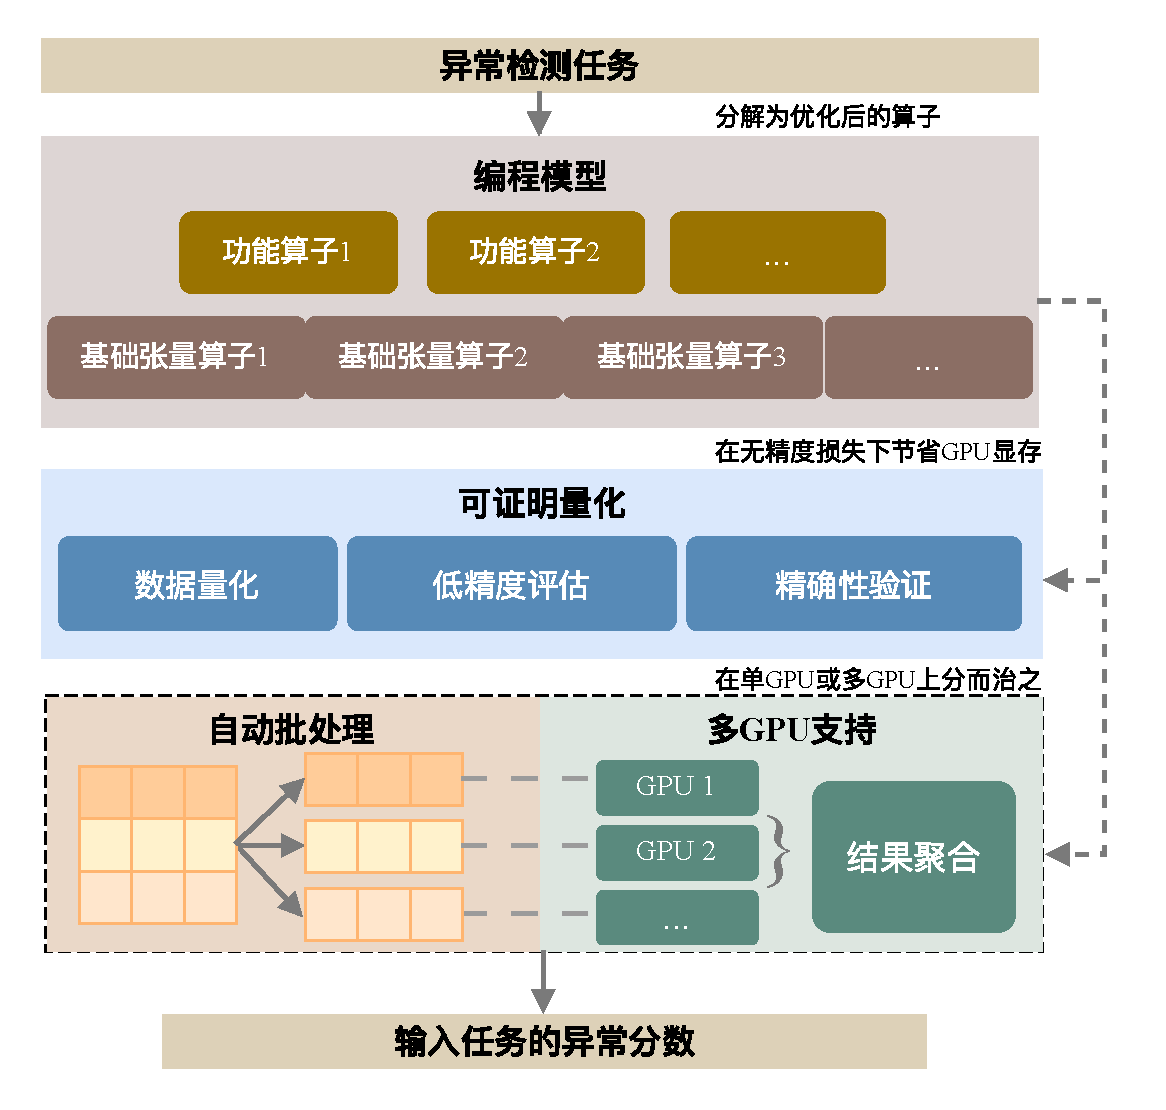
\includegraphics[width=\linewidth]{figures/fig2-1.pdf}
  \caption{TOD 系统总览图（根据文献\citep{zhao2022tod}整理）}
  \label{fig:tod-overview}
\end{figure}

\begin{figure}[!htbp]
  \centering
  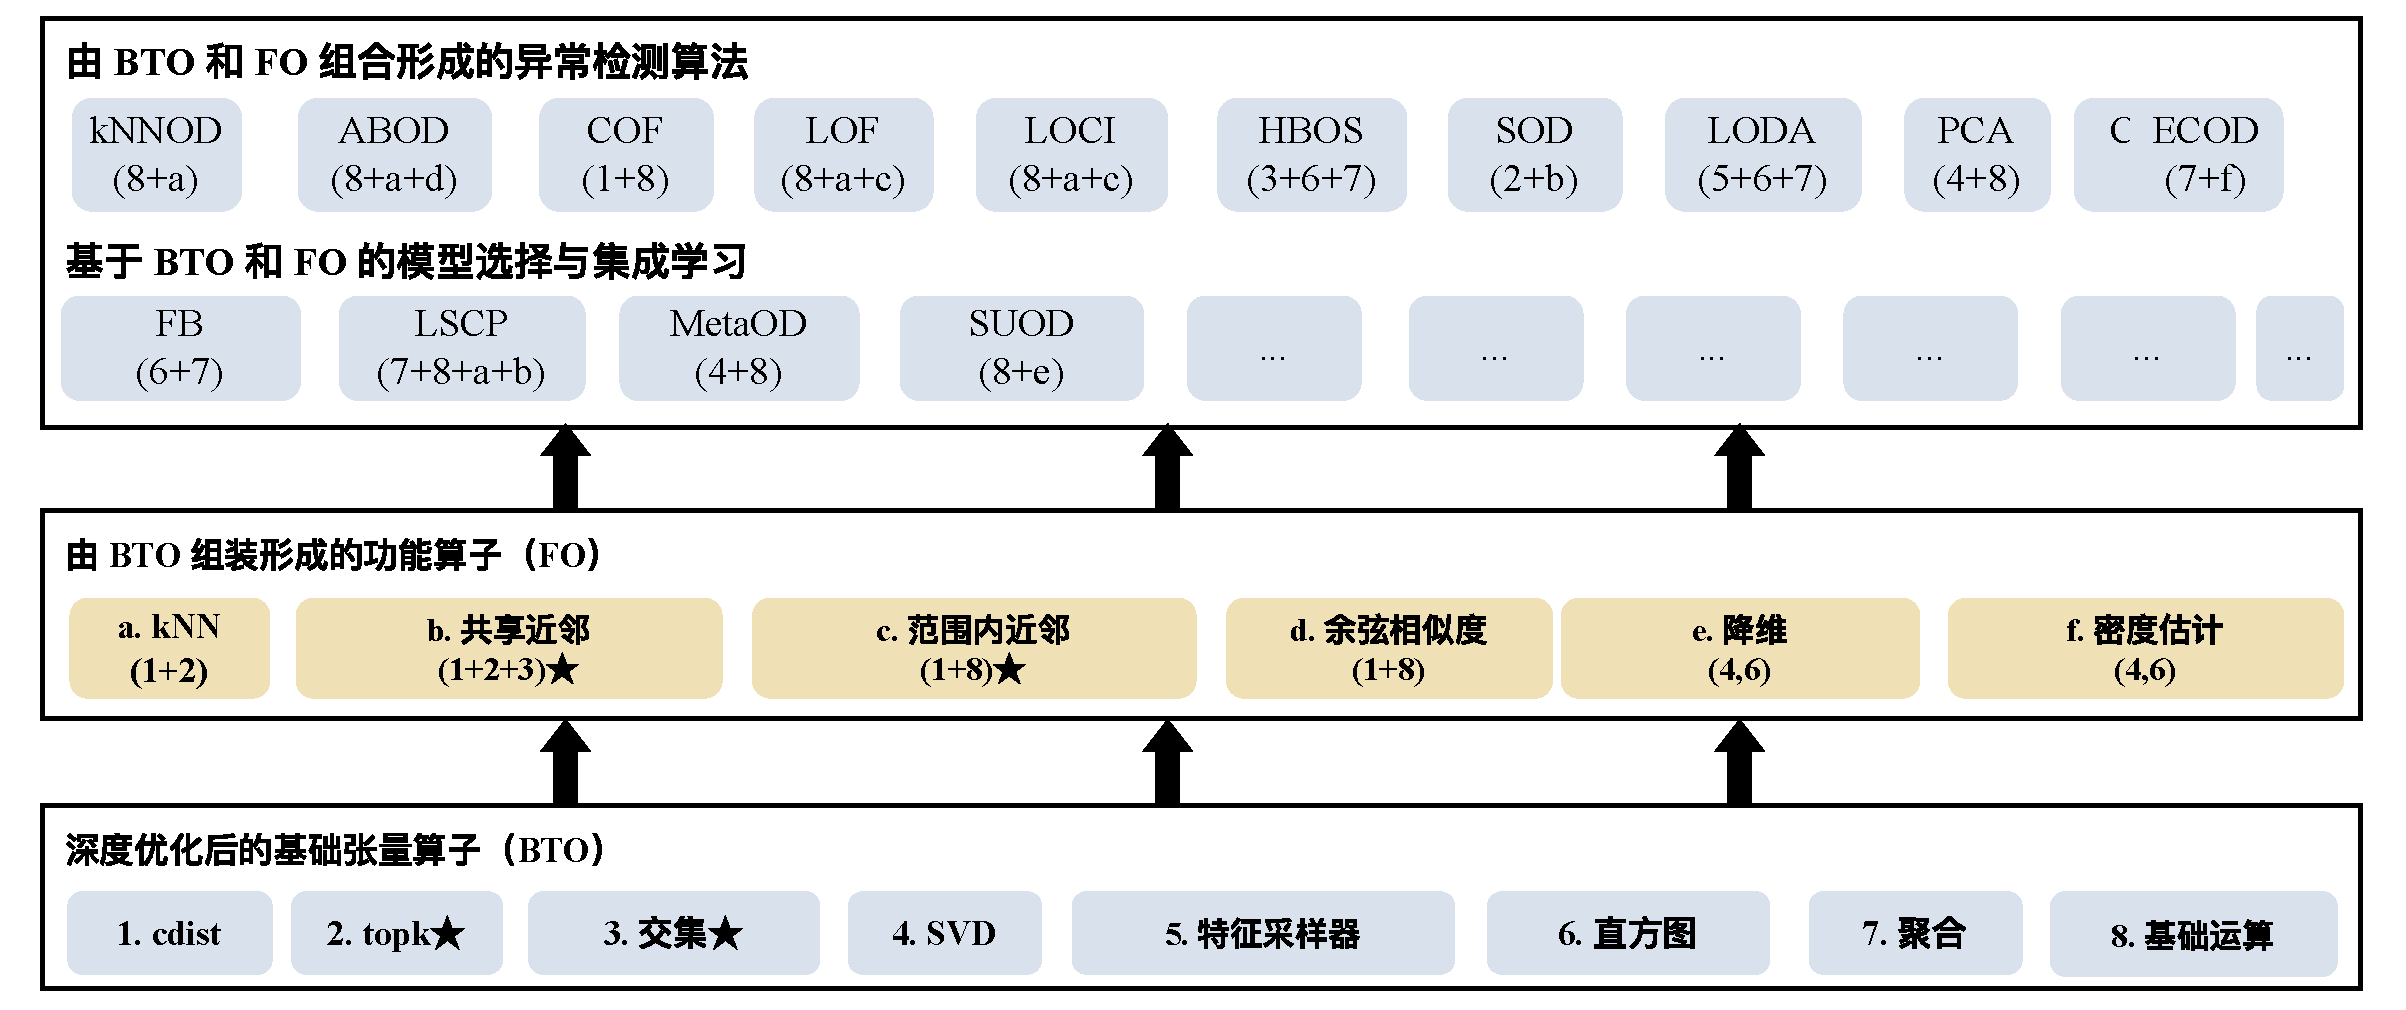
\includegraphics[width=\linewidth]{figures/fig2-2_editable_cn.pdf}
  \caption{典型异常检测算法到张量算子的映射（根据文献\citep{zhao2022tod}整理）}
  \label{fig:algo-to-ops}
\end{figure}

PyTOD 将上述张量化思想提供为可复用的软件接口。本文使用它承接候选集合上的距离、排序和聚合评分，并保留评分函数可替换的空间。早期 GPU 异常检测工作已经证明特定检测器或特征选择步骤可以并行化\citep{angiulli2013gpuoutlier,azmandian2014gpufeature}；TOD/PyTOD 的差别在于提供较统一的算子抽象和批处理执行基础。

它的能力边界也很清楚。PyTOD 不负责从亿级或外存索引中产生候选，不管理 SSD---GPU 访问路径，也不定义候选 ID、distance、local rank 和索引映射如何跨模块传递。在线请求调度与多 GPU 共享 I/O 同样不属于评分框架本身。FlashTOD 因此把 PyTOD 放在候选召回之后：利用其 GPU 评分能力，但不要求它承担前端检索和端到端系统调度。

\section{FlashANNS 近似最近邻候选召回前端}

FlashANNS 是近似最近邻搜索（Approximate Nearest Neighbor Search，ANNS）系统，其功能限于在高维向量索引中返回近邻候选，不输出异常分数。本文把这项能力放在两阶段链路前端：FlashANNS 生成局部候选集合，PyTOD 再根据距离、密度或邻域统计产生异常评分\citep{xiao2025flashanns}。

ANNS 已形成多条技术路线。HNSW 以分层小世界图缩短搜索路径，NSG 通过稀疏导航图控制图规模与遍历代价\citep{malkov2020hnsw,fu2019nsg}；乘积量化（Product Quantization，PQ）用子空间码本压缩向量存储，可与倒排索引等结构组合\citep{jegou2011pq}。当数据超出内存容量后，DiskANN 和 SPANN 分别从 SSD 图索引及内存---外存分层结构处理大规模检索\citep{subramanya2019diskann,chen2021spann}。这些方法的索引结构、内存占用、查询延迟和召回率取舍不同，ANN-Benchmarks 也表明比较结论依赖数据集、参数和评价口径\citep{aumuller2020annbenchmarks}。因此，本文选择 FlashANNS 是为了匹配外存 GPU 候选召回与后续评分链路，并不据此声称它在所有 ANNS 条件下具有普遍优势。

当索引无法完全驻留显存时，搜索过程需要在 SSD 访问与 GPU 计算之间协调。FlashANNS 采用 dependency-relaxed asynchronous I/O，将数据 Fetch、距离 Compute 和候选 Update 交叠推进，并利用 warp 级并发组织细粒度搜索任务。图~\ref{fig:flashanns-io-pipeline}展示了这条流水线。该机制允许部分已就绪计算提前推进，无需等待全部读页完成，从而减少 GPU 的串行等待\citep{xiao2025flashanns,song2026vectoranns}。

\begin{figure}[!htbp]
  \centering
  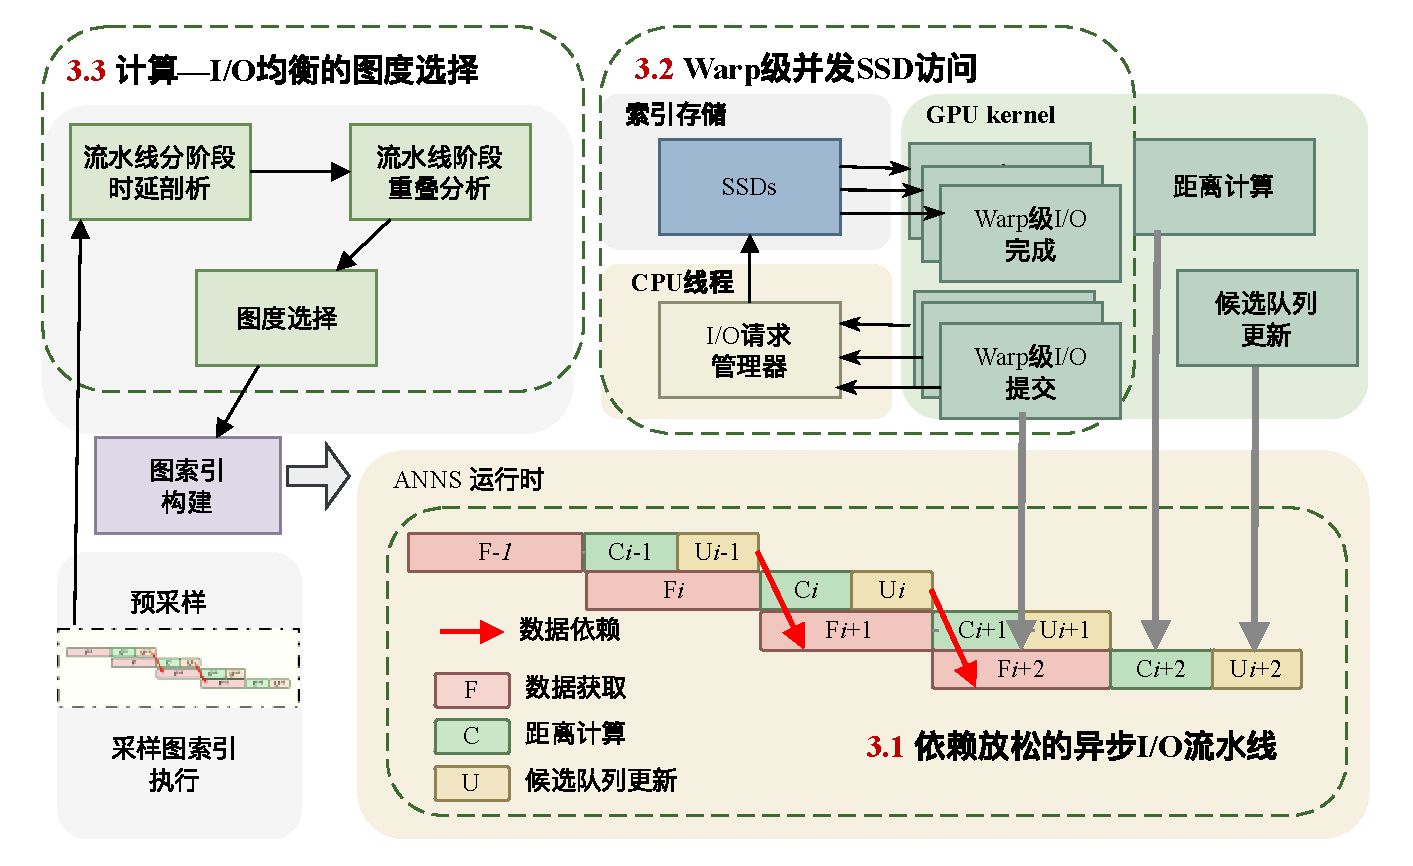
\includegraphics[width=\linewidth]{figures/fig2-3_editable_cn_optimized.pdf}
  \caption{FlashANNS 异步 I/O---计算流水线原理（根据文献\citep{xiao2025flashanns}整理）}
  \label{fig:flashanns-io-pipeline}
\end{figure}

这一能力适合作为 FlashTOD 的候选召回前端，但有三项限制。其一，FlashANNS 只返回近邻候选，异常分数仍由评分模块计算。其二，召回质量依赖搜索深度和候选预算；预算过小可能漏掉评分所需邻域，预算过大会增加后续计算。其三，检索内部的高吞吐不等于端到端高吞吐。若 candidate ID、distance、local rank 和 reference mapping 仍需 D2H 回到 CPU 重组，再经 H2D 送入 PyTOD，阶段边界会重新暴露数据搬运和同步成本。

本文不改写 FlashANNS 的索引或搜索算法。后续工作的切入点是接口组织：使前端输出尽可能保持为设备侧候选缓冲，并与评分张量的布局、批次和生命周期对齐。第四章的数据路径优化由此获得明确问题来源。

\section{单卡数据处理、FAISS-GPU 与接口支撑}

RAPIDS 服务于 GPU 侧数据处理。cuDF 用于字段筛选、类型转换、特征拼接和窗口统计，RMM 为设备内存池及必要的页锁定主机缓冲提供资源管理支持\citep{paul2021dbgpus,rapids_cudf_pandas,rapids_rmm_pinned}。在 FlashTOD 中，这些能力主要用于向量输入准备和候选中间结果组织，不承担异常评分。能否保持全 GPU 执行仍取决于具体操作：兼容模式未覆盖的操作、Python 对象转换或显式主机接口都可能触发 CPU fallback，继而产生额外搬运。第四章需要据实际执行路径检查这些边界。

FAISS-GPU 提供成熟的 GPU ANN API 和资源管理方式，适合验证查询输入与候选输出接口\citep{johnson2019faiss,faiss_gpu_wiki}。同一 GPU 上的 device pointer 可以直接进入索引，避免额外 H2D；host pointer 或跨设备输入则会触发相应数据搬运。其候选 ID、distance 返回格式以及 \texttt{StandardGpuResources} 的 scratch memory 管理，使本文能够在前期确认“检索输出如何进入 PyTOD”这一接口，而不必先依赖完整外存链路。

\begin{figure}[!htbp]
  \centering
  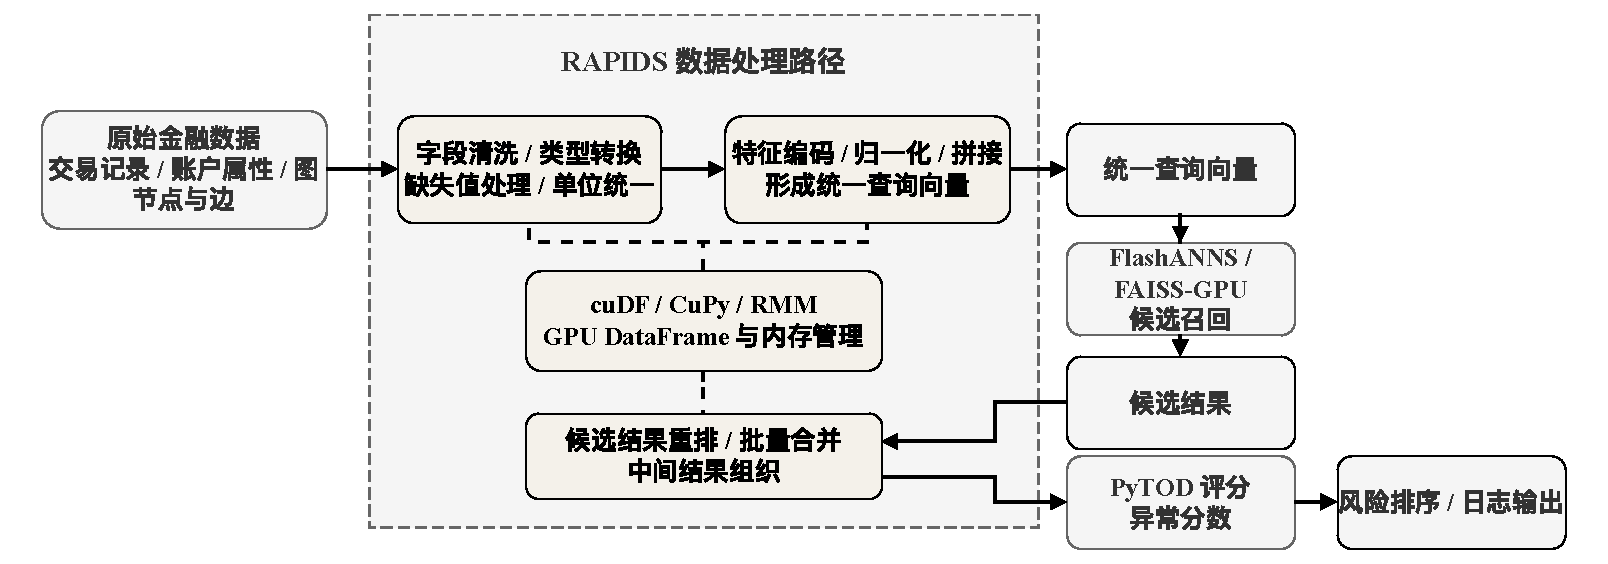
\includegraphics[width=\linewidth]{figures/fig2-4_RAPIDS_position.pdf}
  \caption{RAPIDS 在本文系统中的数据处理位置}
  \label{fig:rapids-position}
\end{figure}

\begin{figure}[!htbp]
  \centering
  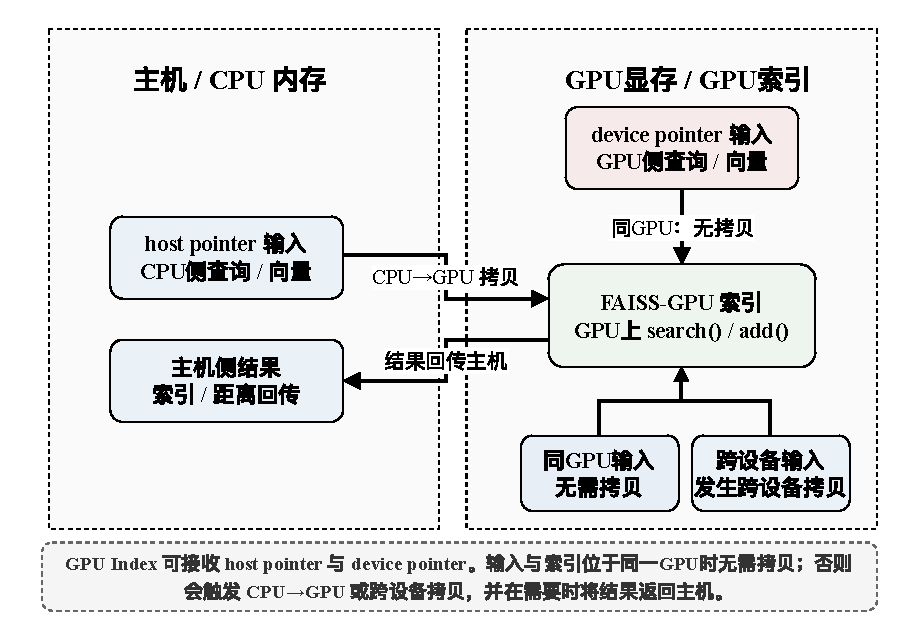
\includegraphics[width=0.8\linewidth]{figures/fig2-5_rapids_faiss_paths.pdf}
  \caption{FAISS-GPU 的 CPU/GPU 互操作路径（根据 FAISS-GPU 文档与本文系统接口整理）}
  \label{fig:faiss-interop}
\end{figure}

三者的边界可以简要概括。RAPIDS 负责数据处理和内存后端，FAISS-GPU 负责前期 ANN 接口及 device/host pointer 路径验证，FlashANNS 负责完整 FlashTOD 中的大规模外存候选召回。完整系统的外存主路径采用 FlashANNS，表格数据处理仍由 RAPIDS 支撑。后续章节直接引用这些角色划分。

\Needspace{0.35\textheight}
\section{多卡调度与在线推理启示}

多 GPU 设计要先在 replicated 与 sharded 之间取舍。replicated 在每张 GPU 上保留完整索引，把不同查询分发给不同设备。查询可以沿用单卡闭环，跨卡通信少，适合索引可复制且吞吐优先的条件；代价是每张卡都要承担索引副本和评分缓冲的显存占用。sharded 将索引分布到多张 GPU，容量扩展更强，但单个查询可能需要访问多个分片并归并局部结果。基于各自适用条件，第五章把 replicated 作为主方案，把 sharded 相关归并放在容量受限时讨论\citep{cuvs_multi_gpu_nn,cuvs_dist_mode}。

归并位置决定 CPU 是否重新进入数据平面。CPU aggregation 实现直接，但各卡局部候选或分数需要 D2H，主机排序后还可能发生 H2D 或额外同步。GPU merge 能保留设备侧结果并减少主机参与，代价是设备间通信、缓冲区管理和 CUDA stream 协调。NCCL 操作可异步入队到指定 stream；同一 \texttt{ncclGroupStart/End()} 中混用多个 stream 可能引入全局同步点\citep{nccl_stream_semantics}。因此，GPU merge 是容量受限路径下需要权衡通信与缓冲管理成本的工程选择。

计算资源增加后，共享 I/O 可能成为上限。多张 GPU 若共享 PCIe switch、NUMA 远端路径或同一 SSD 通道，在途请求会相互排队；GDS 可以减少 CPU bounce buffer，但实际传输仍受 GPU、存储设备与 PCIe 拓扑关系影响\citep{gds_overview,gds_design_guide,li2024multigpunuma}。卡数增加不会自动得到线性吞吐：索引复制占用容量，分片引入归并，CPU 控制面仍需调度请求，共享路径还会抬高 p99 延迟。第五章的 topology-aware I/O 和准入控制正是针对这一限制。

表~\ref{tab:technology-boundary}仅比较文献与成熟技术组件的能力边界。TOD/PyTOD、FAISS-GPU 和 FlashANNS 分别对应 GPU 异常评分、GPU ANN 检索接口和外存 GPU ANNS；FlashTOD 则研究这些能力组合后的候选组织、设备驻留和端到端执行问题。第六章另行区分已有评分方法参考、本文构造的工程组合基线以及内部执行路径对照，各行不构成同口径实验方案。

\begin{table}[!htbp]
  \caption{已有技术能力边界及与本文关系}
  \label{tab:technology-boundary}
  \centering
  \scriptsize
  \setlength{\tabcolsep}{1.0pt}
  \renewcommand{\arraystretch}{1.18}
  \begin{tabularx}{\linewidth}{@{}P{1.70cm}P{1.85cm}C{0.85cm}C{1.35cm}C{0.65cm}C{0.95cm}P{1.60cm}P{1.20cm}Y@{}}
    \toprule
    技术或系统 & 主要研究对象 & 异常评分 & 候选召回 & GPU & 外存 ANNS & 数据路径协同 & 多 GPU & 与本文关系 \\
    \midrule
    传统 CPU 异常检测实现 & CPU 异常评分 & 支持 & 非统一 & 否 & 否 & 主机内执行 & 非统一 & 作为能力参照，本文未新增 PyOD 实验 \\
    TOD/PyTOD\citep{zhao2022tod} & GPU 张量化异常评分 & 支持 & 否 & 支持 & 否 & 评分内部 & 支持 & 第六章以现有全量评分结果作为评分参考 \\
    FAISS-GPU\citep{johnson2019faiss,faiss_gpu_wiki} & GPU ANN 检索与接口 & 否 & 支持 & 支持 & 否 & host/device pointer 接口 & 可扩展 & 作为本文工程组合基线的召回组件 \\
    FlashANNS\citep{xiao2025flashanns} & 外存 GPU ANNS & 否 & 支持 & 支持 & 支持 & 检索内部流水线 & 不作为能力前提 & 本文完整方案的候选召回前端 \\
    本文 FlashTOD & 端到端系统协同 & 经\newline PyTOD & 经\newline FlashANNS & 支持 & 支持 & 研究重点 & 单机多 GPU & 本文完整方案，受数据、硬件和候选预算限制 \\
    \bottomrule
  \end{tabularx}
\end{table}

\section{本章小结}

从现有工作来看，已经提供了 GPU 异常评分、大规模 ANNS、GPU 数据处理和多 GPU 通信能力。需要注意的是，它们针对的是不同层面的问题，各个组件的能力边界要明确，单项能力不会自行组成低开销的端到端系统。

介绍完了现有工作，接下来本文会引出要补充的研究缺口——候选召回与异常评分在统一数据路径中的系统协同。第三章根据这个思路阐述 FlashTOD 的任务模型、模块接口和基础执行流程；第四章再处理功能联通之后仍然存在的候选重组、H2D/D2H 与 I/O 等待问题。
